\documentclass[12pt]{article}
\usepackage{graphicx}
\graphicspath{ {./images/} }
\begin{document}

\section{Week 1 - Linear Regression}
\section{Introduction}
//TODO add references to Coursera ML and Machine Learning for Humans book
We come across  machine learning all the time 

//TODO: add overall outline & what we are intending to cover

It's why I don't have to sift through these emails in my inbox

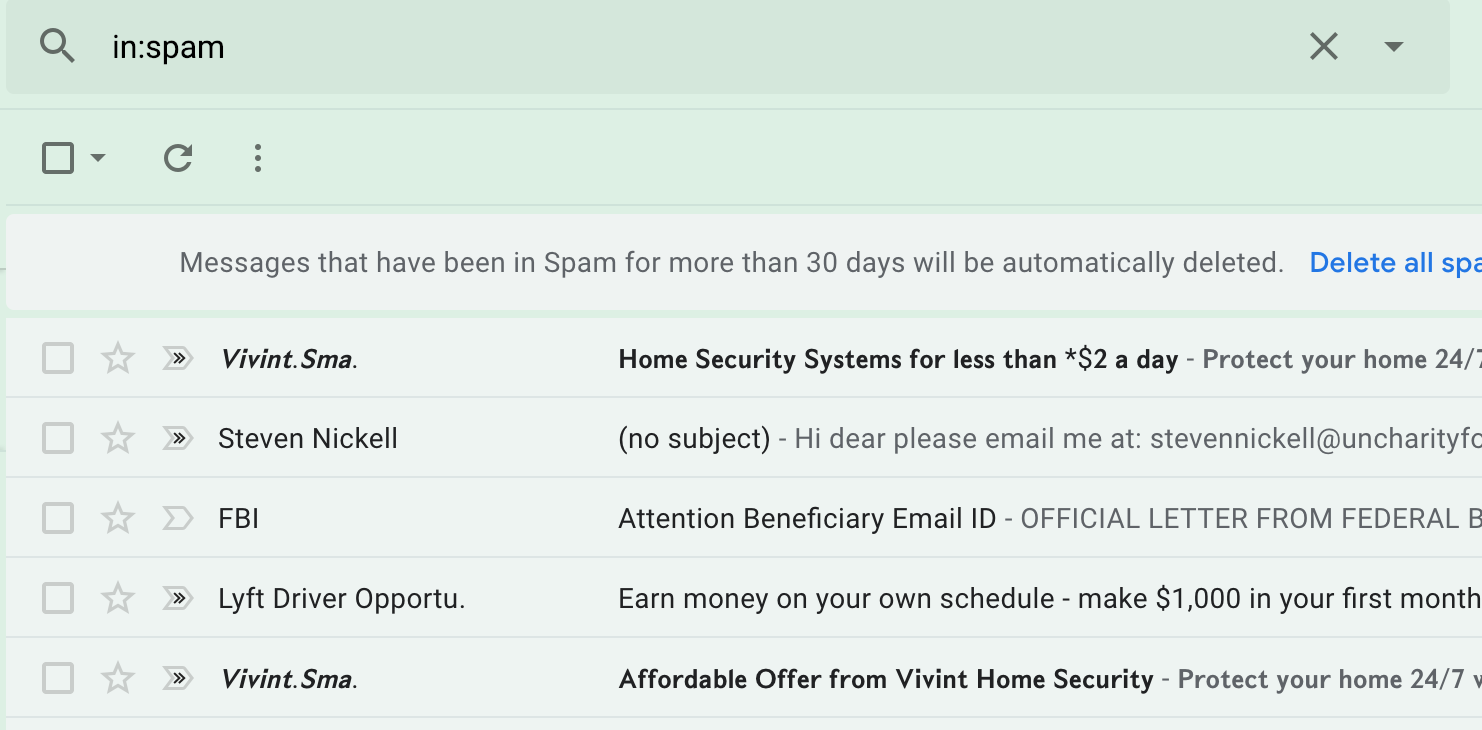
\includegraphics[width=\textwidth]{spam}

It's why I can search my photos, by photos

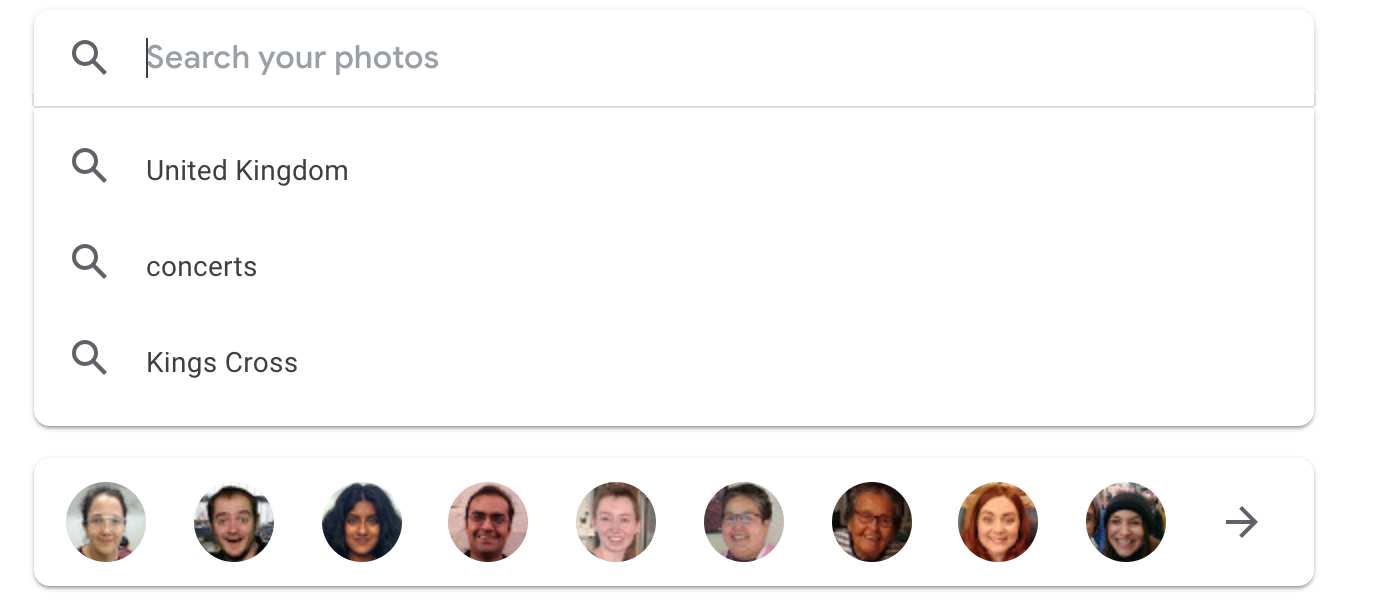
\includegraphics[width=\textwidth]{photo-search}

\subsection{What is Machine Learning?}

According to wikipedia:
Machine learning (ML) is the scientific study of algorithms and statistical models that computer systems use to 
effectively perform a specific task without using explicit instructions, relying on patterns and inference instead.


Machine learning algorithms can learn to do a particular task without being explicitly programmed by building a 
mathematical model based on sample data, known as "training data". Then, that model can be applied to new data 
not previously used to build the model. 

\subsection{What is an algorithm?}

An algorithm is often described as a set of steps to accomplish a particular task. You could describe an algorithm for brushing your teeth, or making a grilled cheese sandwich 

But it's a bit more general than just a set of steps 

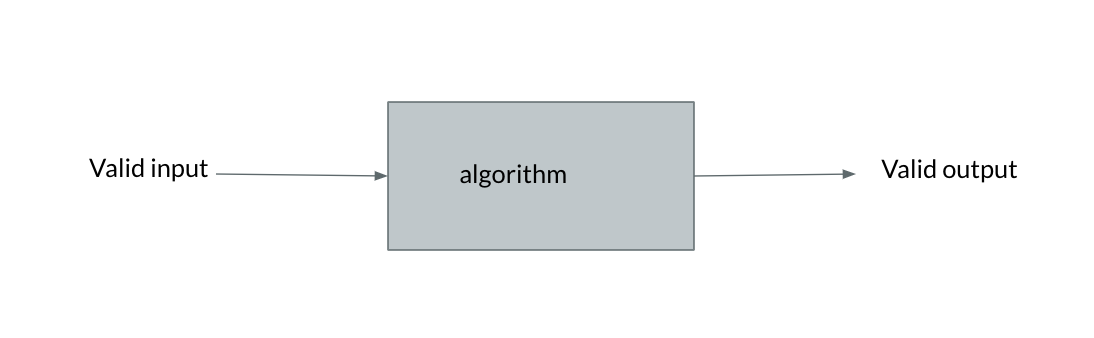
\includegraphics[width={\textwidth}]{algo-abstract}


An algorithm is a way to solve a computational problem, and a computational problem just specifies valid input and desired output. 

For example, for the problem of spam filtering the input would be an email message, and the output would be a 
classification (spam/not spam). The algorithm could be a set of steps. We could compose a series of regular expressions to 
the message that are based on previous messages that we know have turned out to be spam. 

We could also train a model based on a dataset of emails and classifications, to learn patterns of what spam messages 
look like without explicitly writing spam identification rules. Then, we could use the model for new data without a 
classification. That's the approach we're more interested in here, but both approaches are algorithms.

\subsection{What is a machine learning algorithm?}

The ML Coursera course defines a \textit{Well Posed Machine Learning Problem}

A computer program is said to learn from experience $E$ with respect to some task $T$ and some performance measure $P$ 
if its performance on $T$, as measured by $P$ improves with experience $E$

So, we can see that the rule based spam filtering approach wouldn't be a machine learning based approach because having 
more labelled data would not help us to classify spam any more accurately. 

\subsection{Supervised Learning}

Here is an example of a supervised learning problem: 

Suppose we have a dataset of houses that have sold containing how much they have sold for, and the area of the property in square feet. 

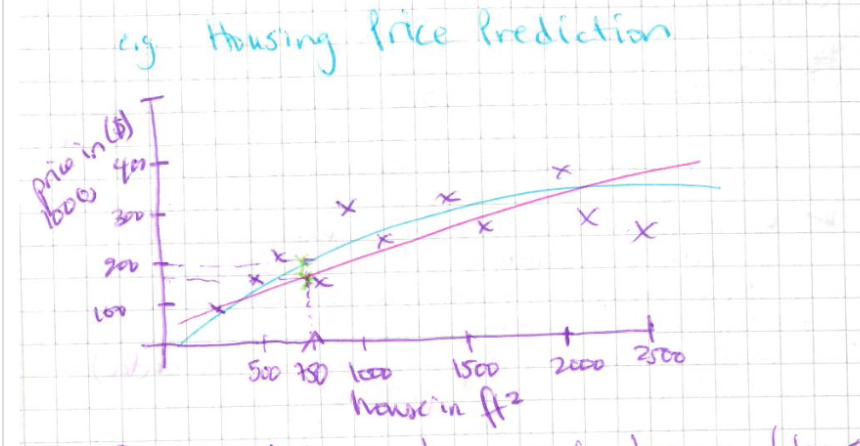
\includegraphics[width={\textwidth}]{housing-prices}

Then, we can use this data to build a model so that we can make a prediction like:

For this new 750 $ft^2$ property, how much will it sell for?

This is a \textit{Supervised Learning} problem because existing labelled data (with the right answers) to work with and to test how accurate our model is. 

This is also a \textit{Linear Regression} problem because the prediction is a continuous valued output. 

Another example of a supervised learning problem would be:

Suppose we want to predict whether a tumour is benign or malignant, and we have a dataset that contains tumours, their size and whether they are benign or malignant.

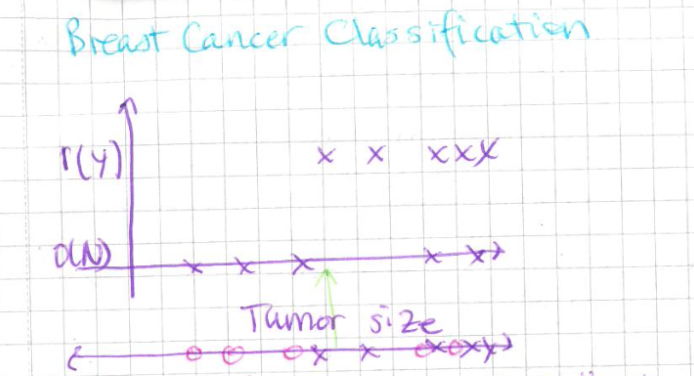
\includegraphics[width={\textwidth}]{tumour-size}

This would be a \textit{classification} problem, because the prediction is a discrete valued output (in this case, either benign or malignant). 

These might seem like toy examples so far. Cancer researchers will collect all sorts of data about tumours and patients that could all be useful in our model. But, we will aim to introduce concepts with a simplified view of the data to help our understanding, then move on to being able to use more features/data and more complicated techniques.

\subsection{Unsupervised Learning}

There is another area of Machine Learning, unsupervised learning that doesn't use labelled data to build a model. We won't cover unsupervised learning here, but let's introduce a couple unsupervised learning problems so that we'll get a feel for what these problems are like, and why they are different from supervised learning.

Here is an example of an unsupervised learning problem:

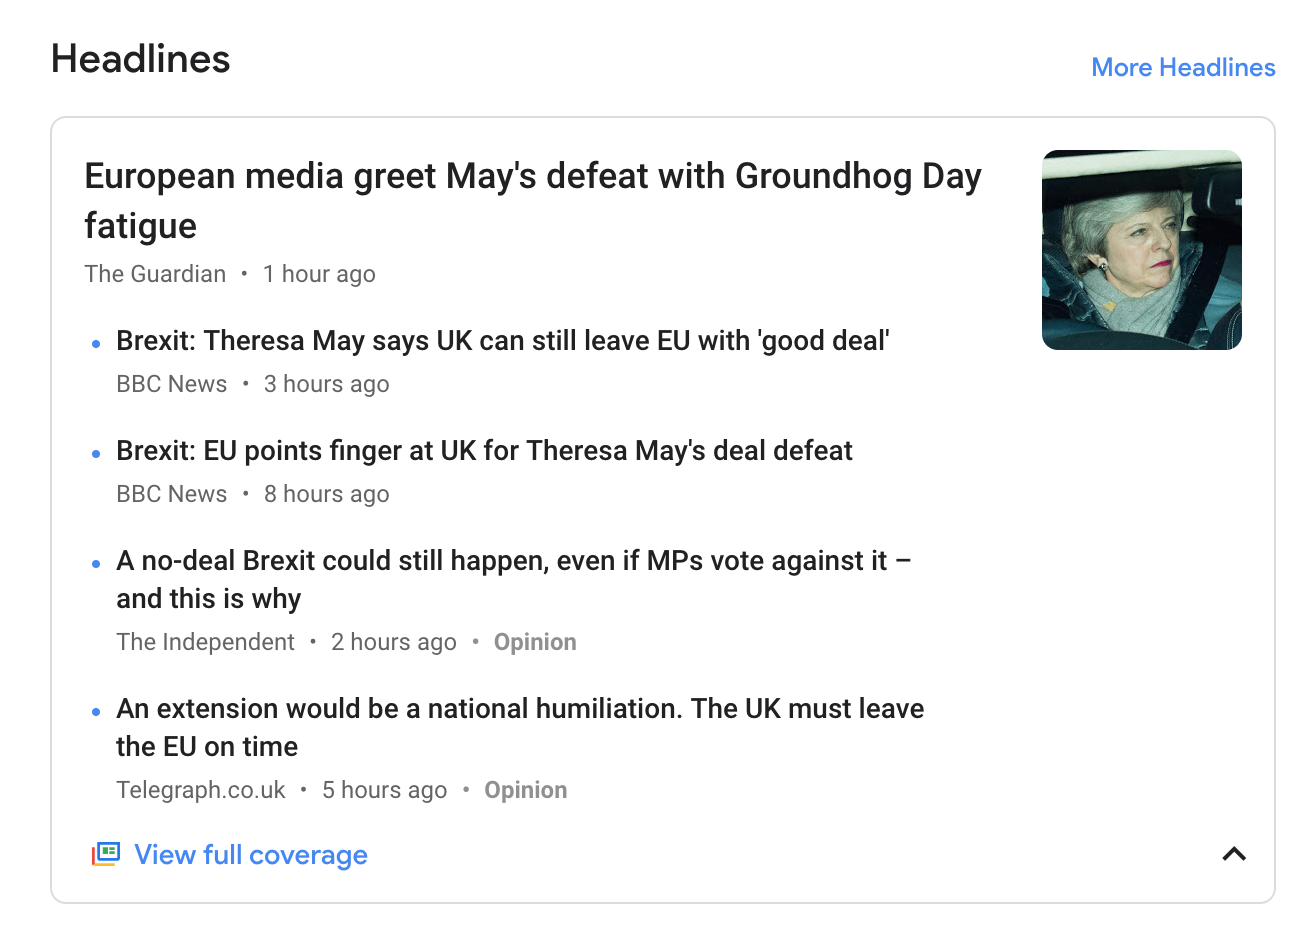
\includegraphics[width={\textwidth}]{google-news}

News aggregators don't have a predefined list of topics, but will find an underlying structure in news articles to be able to group them together, as seen above. 

Here is another example of an unsupervised learning problem:

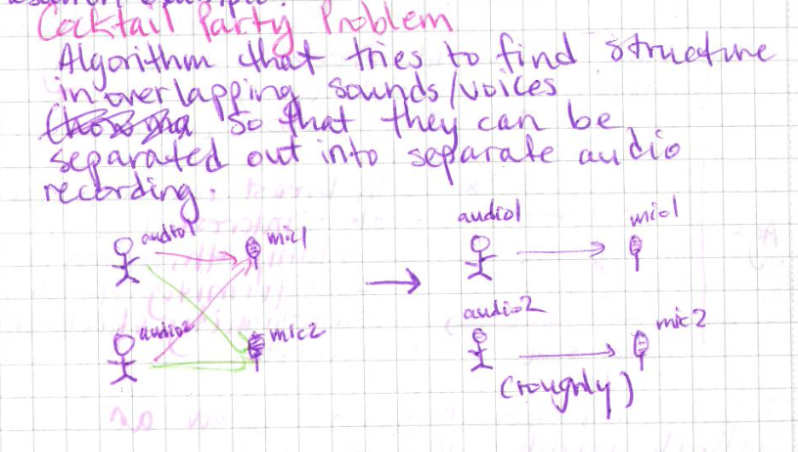
\includegraphics[width={\textwidth}]{cocktail-party}

Given fixed mics in a room, and conversations happening around them, the mics will collect audio data for all of the conversations mixed together. If you want to be able to follow one of the conversations, an algorithm that identifies the underlying structure to be able to extract just the parts of the audio that belong to one conversation is an unsupervised learning problem. 

\subsection{Linear Regression}


\end{document}